\begin{figure}[!h]
\centering
\resizebox{\columnwidth}{!}{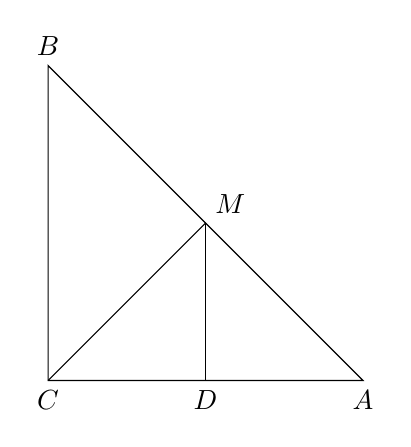
\begin{tikzpicture}
\coordinate (B) at (0,4);
\coordinate (A) at (4,0);
\coordinate (C) at (0,0);
\coordinate (D) at (2,0);
\coordinate (M) at (2,2);
\draw (A)node[below]{$A$}--(B)node[above]{$B$}--(C)node[below]{$C$}--cycle;
\draw(M)node[above right]{$M$}--(D)node[below]{$D$};
\draw(M)--(D);
\draw(M)--(C);
\tkzMarkRightAngle(B,C,A)
\tkzMarkRightAngle(A,D,M)
\tkzMarkRightAngle(C,D,M)
\end{tikzpicture}
}
\caption{Isosceles Triangle with mid-points E and F on equal sides}
\label{eq:solutions/1/16/myfig}
\end{figure}
According to figure \ref{eq:solutions/1/16/myfig}

\begin{align}
\vec{(A-B)}+\vec{(B-F)} &= \vec{(A-F)}\\
\therefore \vec{(B-F)} &= \vec{(A-F)}-\vec{(A-B)}\\
\therefore \vec{(B-F)} &= \frac{1}{2}\vec{(A-C)}-\vec{(A-B)}
\end{align}
similarly,
\begin{align}
\vec{(A-C)}+\vec{(C-E)} &= \vec{(A-E)}\\
\therefore \vec{(C-E)} &= \vec{(A-E)}-\vec{(A-C)}\\
\therefore \vec{(C-E)} &= \frac{1}{2}\vec{(A-B)}-\vec{(A-C)}
\end{align}
Since AB = AC\\
$\therefore (AB)^2 = (AC)^2$\\
\begin{align}
\therefore\norm{\vec{(A-B)}}^2 = \norm{\vec{(A-C)}}^2
\end{align}
\begin{multline}
\norm{\vec{(A-B)}}^2+\frac{1}{4}\norm{\vec{(A-C)}}^2 -\vec{(A-C)}^T\vec{(A-B)} =\\
\norm{\vec{(A-C)}}^2+\frac{1}{4}\norm{\vec{(A-B)}}^2 -\vec{(A-B)}^T\vec{(A-C)} \end{multline}
\begin{multline}
\brak{\frac{1}{2}\vec{(A-C)}-\vec{(A-B)}}^T\brak{\frac{1}{2}\vec{(A-C)}-\vec{(A-B)}}=\\
\brak{\frac{1}{2}\vec{(A-B)}-\vec{(A-C)}}^T\brak{\frac{1}{2}\vec{(A-B)}-\vec{(A-C)}}
\end{multline}
\begin{align}
\norm{\vec{(B-F)}}^2 &= \norm{\vec{(C-E)}}^2\\
\therefore\norm{\vec{B-F}} &= \norm{\vec{C-E}}
\end{align}
Hence, BF is equal to CE
